\documentclass[pdf, slideColor]{beamer}
\usepackage[czech]{babel}
\usepackage[utf8]{inputenc}
\usepackage[T1]{fontenc}
\usepackage{picture}
\usepackage{graphicx}
\usepackage{color}
\usepackage{gensymb}
\usetheme{Berkeley}
\usecolortheme{beetle}

\providecommand{\uv}[1]{\quotedblbase #1\textquotedblleft}

\begin{document}
	\title{Vesmír}
	\subtitle{Zajímavosti, o kterých jste nevěděli}
	\author{Tomáš Aubrecht}
	\date{\today}
	\maketitle

\begin{frame}{Hvězdy}
\smallskip
\textbf{Wise 1828+2650}
	\begin{itemize}
		\item nazývána hvězdou hnědého trpaslíka
		\item průměrné teploty se pohybují v rozmezí $-127\celsius$ až $-23\celsius$ \smallskip
	\end{itemize}
\textbf{BMP 37093}
	\begin{itemize}
		\item jádro tvořené diamanty, které mají 10 miliard bilion bilionů karátů\smallskip
	\end{itemize}
\textbf{Neutronové hvězdy}	
	\begin{itemize}
		\item jejich hustota je tak obrovská, že 1 lžíce jejich hmoty by vážila přes 100 milionů tun\smallskip
\end{itemize}
\end{frame}

\begin{frame}{Černá díra}
\smallskip
\begin{itemize}
    \item objekt natolik hmotný, že jeho gravitační pole je v jisté oblasti časoprostoru natolik silné, že žádný objekt včetně světla nemůže tuto oblast opustit \smallskip
    \item byla teoreticky předpovězena Albertem Einsteinem \smallskip
    \item nemůžeme ji pozorovat přímo, proto není stanoveno korektně nic včetně její data objevu
\end{itemize}
\end{frame}

\begin{frame}{Kolonie na Marsu}
\smallskip
\textbf{\uv{Mars One}} \smallskip
\begin{itemize}
	\item organizace snažící se vytvořit stálou kolonii na Marsu
    \item přihlásilo se přes 200 000 dobrovolníků, z nichž byli vybráni pouze 4
    \item v roce 2026 odstartuje první posádka, která by po 7 měsících měla přistát na Marsu
	\item potom každé 2 roky by měly být další lety na Mars
\end{itemize}
\end{frame}

\begin{frame}{Barva Slunce}
\smallskip
\begin{itemize}
    \item není žlutá, ale pouze se tak jeví díky zemské atmosféře \smallskip
    \item sluneční paprsky obsahují všechny barvy viditelného barevného spektra, které mají přibližně stejnou intenzitu, proto je ve skutečnosti \textbf{bílá}
\end{itemize}
	

\begin{center}
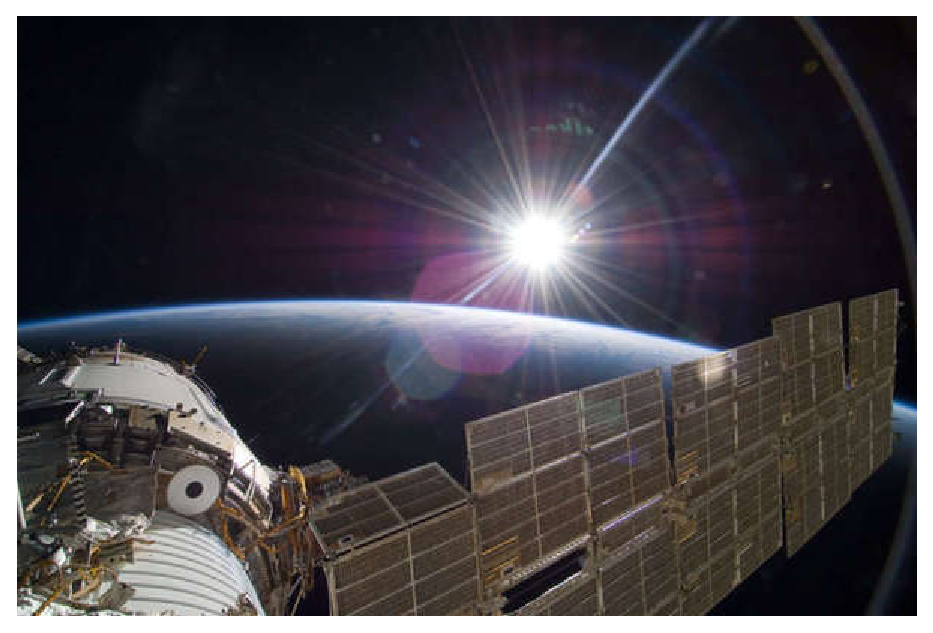
\includegraphics[scale=0.3]{slunce}\\
\end{center}

\end{frame}

\begin{frame}{Trpasličí planeta}
\smallskip
\begin{itemize}
	\item  je objekt sluneční soustavy, který:
	\begin{itemize}
		\item obíhá okolo Slunce
		\item má dostatečnou hmotnost, aby jeho gravitace překonala vnitřní síly a dosáhl hydrostatické rovnováhy
		\item během svého vývoje nepročistil své okolí, aby se stal v dané zóně dominantní
		\item není satelitem
	\end{itemize}
	\item kromě Pluta, které již není nadále považváno za planetu, existují i jiné \uv{planetky} jako: \smallskip
	\begin{itemize}
		\item Ceres
		\item Eris
		\item MakeMake
		\item Haumea
		\item Quaoar
	\end{itemize}
\end{itemize}
\end{frame}

\begin{frame}{Venuše}
\smallskip
\begin{itemize}
	\item jako jediná planeta se otáčí okolo své osy v opačném smyslu, než ve kterém obíhá kolem Slunce
	\item oběh kolem Slunce trvá 224 pozemských dní, rotace kolem své osy trvá 243 dní
	\item hvězdný den na Venuši je \textbf{delší} než Venušin rok 
\end{itemize}
\begin{center}
	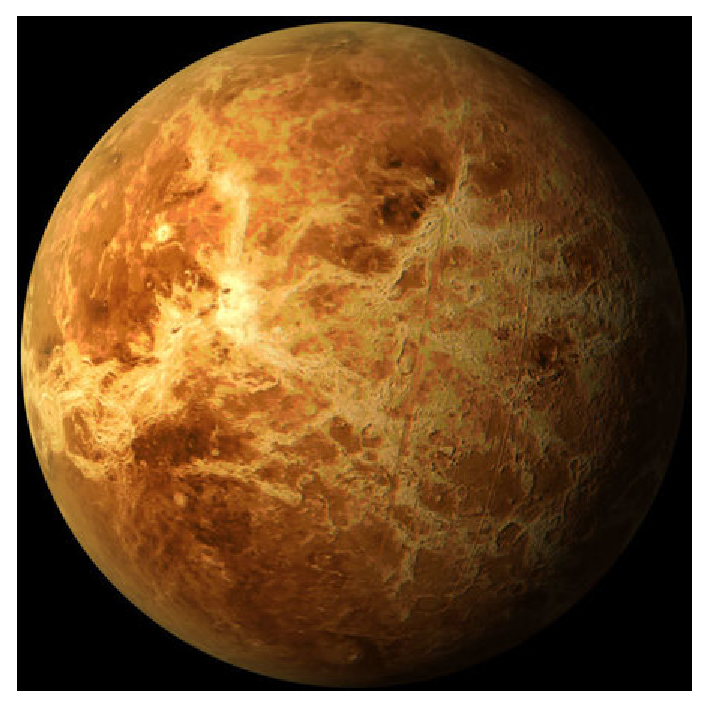
\includegraphics[scale=0.25]{venuse}\\
\end{center}
\end{frame}

\begin{frame}{Zdroje}
\begin{itemize}
	\item Youtube: 
	\begin{itemize}
		\item https://www.youtube.com/watch?v=W62aVty77Lw
		\item https://www.youtube.com/watch?v=lOmZnqeeySg
		\item https://www.youtube.com/watch?v=I5CBrjpnSNo
	\end{itemize}
	
	\item Wikipedia: 
		\begin{itemize}
		\item https://en.wikipedia.org/wiki/Universe
		\item https://en.wikipedia.org/wiki/Mars
		\item https://en.wikipedia.org/wiki/Planet
	\end{itemize}
	
\end{itemize}
\end{frame}

\end{document}